% !TEX TS-program = pdflatex
% !TEX encoding = UTF-8 Unicode

% This is a simple template for a LaTeX document using the "article" class.
% See "book", "report", "letter" for other types of document.

\documentclass[11pt]{article} % use larger type; default would be 10pt

\usepackage[utf8]{inputenc} % set input encoding (not needed with XeLaTeX)

%%% Examples of Article customizations
% These packages are optional, depending whether you want the features they provide.
% See the LaTeX Companion or other references for full information.

%%% PAGE DIMENSIONS
\usepackage{geometry} % to change the page dimensions
\geometry{a4paper} % or letterpaper (US) or a5paper or....
% \geometry{margin=2in} % for example, change the margins to 2 inches all round
% \geometry{landscape} % set up the page for landscape
%   read geometry.pdf for detailed page layout information

\usepackage{graphicx} % support the \includegraphics command and options

% \usepackage[parfill]{parskip} % Activate to begin paragraphs with an empty line rather than an indent

%%% PACKAGES
\usepackage{booktabs} % for much better looking tables
\usepackage{array} % for better arrays (eg matrices) in maths
\usepackage{paralist} % very flexible & customisable lists (eg. enumerate/itemize, etc.)
\usepackage{verbatim} % adds environment for commenting out blocks of text & for better verbatim
\usepackage{subfig} % make it possible to include more than one captioned figure/table in a single float
% These packages are all incorporated in the memoir class to one degree or another...

%%% HEADERS & FOOTERS
\usepackage{fancyhdr} % This should be set AFTER setting up the page geometry
\pagestyle{fancy} % options: empty , plain , fancy
\renewcommand{\headrulewidth}{0pt} % customise the layout...
\lhead{}\chead{}\rhead{}
\lfoot{}\cfoot{\thepage}\rfoot{}

%%% SECTION TITLE APPEARANCE
\usepackage{sectsty}
\allsectionsfont{\sffamily\mdseries\upshape} % (See the fntguide.pdf for font help)
% (This matches ConTeXt defaults)

%%% ToC (table of contents) APPEARANCE
\usepackage[nottoc,notlof,notlot]{tocbibind} % Put the bibliography in the ToC
\usepackage[titles,subfigure]{tocloft} % Alter the style of the Table of Contents
\renewcommand{\cftsecfont}{\rmfamily\mdseries\upshape}
\renewcommand{\cftsecpagefont}{\rmfamily\mdseries\upshape} % No bold!

%%% END Article customizations

%%% The "real" document content comes below...

\title{\textbf{Air Quality in China: Explorations}}
\author{Shengqian Chen, Alex Dewey, Ruoying Jiang, Xingxing Tong}
%\date{} % Activate to display a given date or no date (if empty),
         % otherwise the current date is printed 

\usepackage[font=small,labelfont=it]{caption}


\begin{document}
\maketitle

\begin{abstract}
Air pollution is a major cause of mortality, disease and disability in China.
Even extremely conservative estimates suggest that air pollution may have an 
premature death toll of 350,000-500,000 people per year in China alone,
and there are several other health risks associated with air pollution which reduce quality of life. 
Some of the most important forms of air pollution are the so-called \textit{fine particles}, aerosol particles
less than 2.5 micrometers in diameter, which arise from burning fossil fuels, as in
industrial, household, and transit settings.

In this report, we variously explore the U.S. State Department's ``Mission China'' dataset, which 
collects hourly data on fine particulate (or \(PM_{2.5}\)) in five major urban centers of China. First, we look at the hourly and locational
nature of the data. Then we use regression and meteorological data to explore what proximate weather-related
factors most have the most direct effect on air pollution in Beijing. Finally, we suggest
directions for future exploration.
\end{abstract}

\section{Introduction}

\subsection{Air Pollution}
\begin{figure}[!ht]
  \centering
    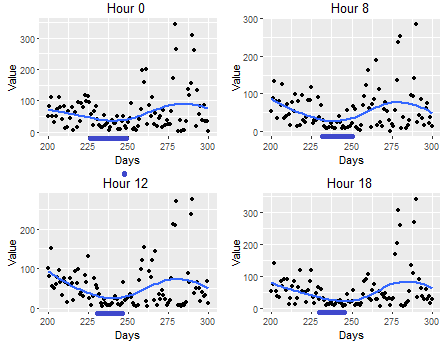
\includegraphics[width=0.6\textwidth]{ParadeBlueBeijing}
      \caption{Decreased air pollution (by \(\mathit{PM_{2.5}}\)) during Beijing's Parade Blue, at four different times of day.
      Note that Day 250 is September 7}
\end{figure}


Air pollution is a major cause of mortality, disease and disability in China.\cite{Yang10, Stein14} 
According to a 2013 study published in the Lancet \cite{Yang10}, ambient and household
air pollution in 2010 accounted for China's fourth- and fifth-largest risk factors
in terms of lost disability-adjusted life years (DALYs)\cite{WHO16}.
Even conservative estimates, such as that given by former Health minister Chen Zhu
in 2013\cite{Moore14}, peg the death toll at between 350,000 and 500,000 deaths per year.
A think tank surveying the literature estimated
that between 1.2-2 million premature deaths may be attributable to air pollution annually in China\cite{Rohde15}. 

Aerosol particles, especially \textit{fine particles} of less than 2.5 micrometers (or \(PM_{2.5}\)),
are so deadly because they exacerbate some of the
most common causes of death and ill health: Particle pollution has been linked with "premature death 
in people with heart and lung disease, nonfatal heart attacks, irregular heartbeat,
aggravated asthma, decreased lung function, and increased respiratory symptoms," per the EPA\cite{EPA16}. 

In August 2015, the Chinese government halted much of the country's
industrial capacity and traffic for a WWII 70th anniversary celebration called "Parade Blue"\cite{Boren15}.
During Parade Blue, \(PM_{2.5}\) readings quickly 
dropped to record lows, dropping below 19.5 and averaging 
\(35 \mu g/m^3\) during the celebration, well below typical readings. 
Once the celebration ended, however,
\(PM_{2.5}\) readings gradually returned to their historical norms. Parade Blue demonstrates
starkly how sensitive air pollution is to proximate human activities
and to their reduction.

\subsection{Key Questions}

The U.S. Department of State collects hourly data in five cities at the Beijing Embassy
and four other Consulates in large metropolitan areas (Guangzhou, Shanghai, Chengdu, and
Shenyang). According to 2010 Census data, the combined population of these 5 cities' administrative areas is greater than
100 million people (or some 1.5\% of the human population 
and 7\% of the population of China)\cite{Wiki16}.

Air pollution is caused by human activity
such as industry, heating (especially solid fuels such as coal and wood used in household heating and cooking),
and transportation, and cities, being a concentrated mass of human activies, are an obvious starting point
in China's efforts to improve air quality. Lacking the domain knowledge to mount a proper study, we
instead decided to look at collating and presenting what information was available to us---
not only what we could find in the State Department's data but also other publicly-available datasets.

In particular, we decided to look at time-and-location indexed, meteorological, and climatological data,
in order to figure out which obvious factors might play a role in successfully understanding air pollution.

More information will be provided in the section on Data Sources, 
but, for some basic reference points, all our air quality data is measured in terms of 
\(PM_{2.5}\), which measures the 
total mass of fine particles in the atmosphere (micrograms
per cubic meter). Anything below 35.4 \(\mu g/m^3\) is considered
Good or Moderate, while readings between 35.4 to 55.4 are ``Unhealthy for Sensitive Groups,''
55.4 to 150.4 is Unhealthy, up to 250.4 is Very Unhealthy, and anything above 250.4  \(\mu g/m^3\)
is considered Hazardous.





\section{Exploratory Plotting}

	As mentioned above, our dataset comes from the U.S. Department of State in the Embassy and Consulates of five major cities in China. Data is measured in terms of the total mass of particulate matter (particles with size 2.5 micrometers or less, which we denote as " \(PM_{2.5}\)"). The  \(PM_{2.5}\) data is hourly over the course of 2015, so there are 24 data points in each day for each of the five cities.

	The goal of this part of our analysis is to explore the raw dataset based on visualization. We hope to get a big picture about the distribution of  \(PM_{2.5}\) among these five cities. Numerical analysis will be conducted in the next part.
	
\begin{figure}[!ht]
  \centering
    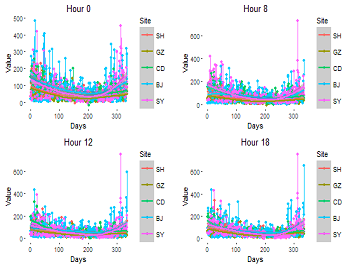
\includegraphics[width=0.8\textwidth]{Figure1-1}
      \caption{Each plot is the value of everyday \(PM_{2.5}\) at a particular time point (12:00 am, 8:00 am, 12:00 pm, and 6:00 pm) in 5 big cities in China (Shanghai, Guangzhou, Chengdu, Beijing, and Shenyang).
}
\end{figure}

	The nature of this dataset (and personal experience with air pollution) led us to a hypothesis that the pattern of \(PM_{2.5}\) varies from hour to hour, especially around peak driving hours. So we focused on four specific hours in the first stage of our exploration: We collected data at 12:00am, 8:00 am, 12:00 pm, and 6:00pm. 8:00 am and 6:00 pm are chosen since they are rush hours where we expect to see primary levels of transportation, 12:00am seems to be a solid baseline for low human activity, and 12:00 pm is the midday, where we might expect lower transportation but higher industrial air pollution.
	
\begin{figure}[!ht]
  \centering
    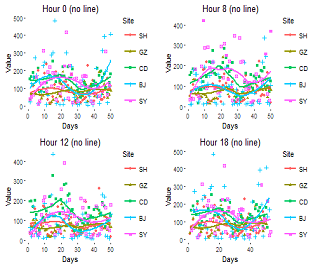
\includegraphics[width=0.6\textwidth]{Figure1-2}
      \caption{Four time-of-day plots of 5 cities for the first 50 days}
\end{figure}

	Based on an informal comparison of these four hours, we made the assumption that the \(PM_{2.5}\) would be highly correlated with air pollution from traffic. We therefore expected to see relatively low \(PM_{2.5}\) at 12:00am and relatively high values at the 8:00 am and 6:00pm measurements.

	In Figure 2 is our  \(PM_{2.5}\) plot for all five cities at the four hours. Note that the graph is color-coded by site: SH means Shanghai, GZ is Guangzhou, CD indicates Chengdu, BJ is Beijing, and SY stands for Shenyang. 
	


	The density of points in Figure 2 (above) from these five cities makes it hard to notice any pattern. So, as an exploration, we decided to focus the first 50 days of 2015 which gives us the following graph.
	


In order to make the pattern for each city manifest more clearly, we concentrate on Hour 0 and split cities apart. 

\begin{figure}[!bt]
  \centering
    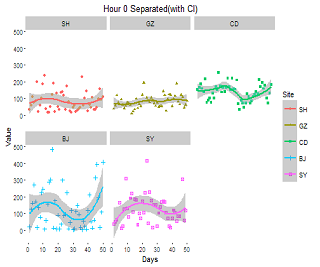
\includegraphics[width=0.8\textwidth]{Figure1-3}
      \caption{Hour 0 plots of 5 cities for the first 50 days}
\end{figure}

Figure 3 above indicates that for the given hour and day period, Shanghai and Guangzhou maintain a very stable pattern. The \(PM_{2.5}\) for Chengdu fluctuates a bit, but its pattern remains stable in general. For Beijing and Shenyang, however, their  \(PM_{2.5}\) values change violently over the first 50 days. Different latitudes and longitude mays provide some of the explanation for this, as Shanghai and Guangzhou are in the south of China, while Beijing and Shenyang are in the north. 
	There is a clear upward trend for Beijing in this 50-day interval. It seems that the \(PM_{2.5}\) values for Beijing are higher than for other cities on average for the following days. This intuitive analysis gives us an indication that it might be most interesting to explain the data for Beijing.

\newpage

\section{Regression Fitting and Outlier Analysis}
\subsection{Regression of meteorological factors on daily average \(PM_{2.5}\)}

In general, academic papers\cite{Chatani11, Tai10, Pohjola02} suggest that three major factors contribute to the concentration of \(PM_{2.5}\): 1. domestic sources of emissions, 2. foreign sources, and 3. meteorological conditions.

As Pohjola \textit{et al.} note: “[M]eteorological conditions can largely diffuse, dilute, and accumulate pollutants.”\cite{Pohjola02}. Tai \textit{et al.} make an even stronger claim: “We find that daily variation in meteorology as described by the multiple linear regression can explain up to 50\% of \(PM_{2.5}\) variability with temperature, relative humidity, precipitation, and circulation all being important predictors.”\cite{Tai10}.
 
Thus, in the second part of our project, we explore the relationship between meteorological variables and daily mean \(PM_{2.5}\) values for each day in 2015. 
Based on the analysis in the Exploratory Plotting section on the first 50 days of 2015, Beijing---the capital and political center of China---is somewhat outstanding in its \(PM_{2.5}\) data, presenting a higher level of emissions in general than in the other four cities.

As mentioned in the Data Sources section, all the meteorological data we obtained is from the Weather Underground website. So that our metereological data accords with our air pollution data, we consider the mean daily value for all of our factors (temperature, dew point, humidity, sea level pressure, and wind speed). We have this data for each day from January 1 to December 31, 2015. In order to take the time series of our data into account, we also include the prior day's mean \(PM_{2.5}\).

 \begin{figure}[!ht]
  \centering
    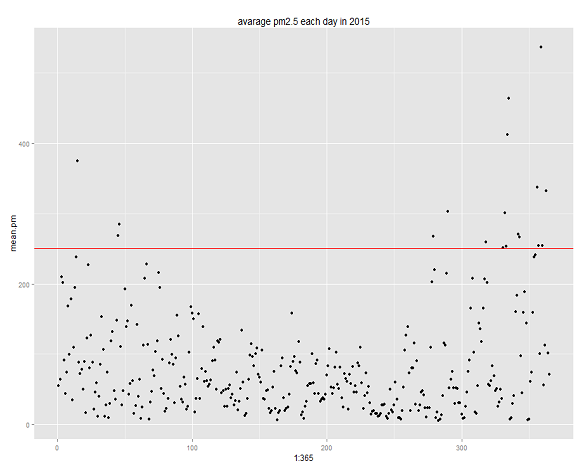
\includegraphics[width=0.65\textwidth]{Figure2-1}
      \caption{Daily average of \(PM_{2.5}\) measurements in Beijing for each day of 2015. The red line is at the value 250 \(\mu g / m^3\). We delete points above the red line in our model fitting.}
\end{figure}

Having collected this data, we combined the meteorological data with the daily average\(PM_{2.5}\) data, then attempted to fit a regression model which would explain air pollution on each day. However, after drawing a graph of daily average \(PM_{2.5}\) during 2015, we noticed that the daily \(PM_{2.5}\) means have considerably higher means and a large number of outliers at the beginning and end of the year. In order to minimize the impacts of these extreme outliers on our final model, we decided to start by focusing only on days with relatively normal levels of \(PM_{2.5}\). According to the new air quality standards in China, we delete days that have average \(PM_{2.5}\) higher than 250\(\mu g/m^3\). Each of these deleted days represents a day marked by severe pollution. For 2015, Beijing has 18 days where the measured \(PM_{2.5}\) is larger than \(\mu g/m^3\).


 
 
Once these outliers are set aside, we attempt a multiple linear regression without interaction terms. We'll return to the outliers later. 

\subsubsection{Regression Results} 
When we include all meteorological variables and one lag factor, we find that only four variables appear to be significant: The daily average values of temperature, sea level pressure, wind speed and the lag factor of the previous day's emissions. In Table 1 below, we summarize the results of this regression.
 
 \begin{table}
 \begin{tabular} {| r | r | r | r | r |}
 \hline
 \textbf{Variable} & 
\textbf{Estimated} & 
\textbf{Standard Error} & 
\textbf{t-value} \(\mathbf{t_0}\) & 
\(\mathbf{Pr(\vert t_0 \vert >t)}\) \\ \hline
\textbf{Intercept} & 1561.10 & 409.78 & 3.810 & 1.65 E-4 \\ \hline
\textbf{Lagged }\(\mathbf{PM_{2.5}}\) & 0.4485 & 0.0389 & 11.527 & \(<\)2 E-16 \\ \hline
\textbf{Temperature} & -1.20870 & 0.21537 & -5.612 & 4.14 E-8 \\ \hline
\textbf{Pressure (Sea Level)} & -46.729 & 13.278 & -3.519 & 4.91 E-4 \\ \hline
\textbf{Wind Speed} & -8.56 & 0.69 & -12.404 & \(<\)2 E-16 \\ \hline
 \end{tabular}
 \caption{Significant variables in the linear model.}
 \end{table}
 
Based on Table 1 (below), the estimated coefficients of 
mean temperature, mean sea level pressure and mean wind speed for each day are negative, 
which indicates negative effects of increasing these
meteorological variables on the \(PM_{2.5}\) values. 
By contrast, the positive coefficient of our one-day lag term suggests a positive relationship between
\(PM_{2.5}\) and the lagged response.

Is this model successful? The adjusted R-squared is 0.5116, which is weaker than we might want considering the previous day's mean is included and indicates the fitted model is not ideal. 
In Figure 7 (left), we see that the residuals increase with the fitted value. Together, these facts suggest we should look for an appropriate transformation of the data.

\begin{figure}
\centering
\begin{minipage}{.5\textwidth}
  \centering
  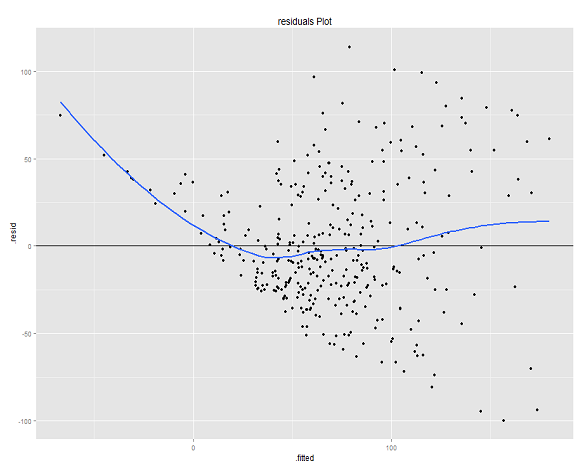
\includegraphics[width=\linewidth]{Figure2-2}
  \label{fig:test1}
\end{minipage}%
\begin{minipage}{.5\textwidth}
  \centering
  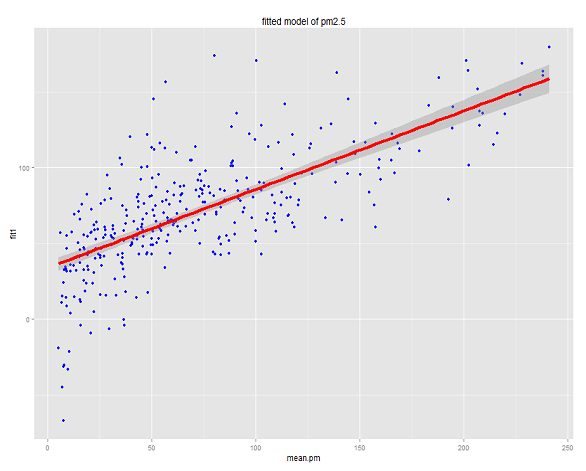
\includegraphics[width=\linewidth]{Figure2-3}
  \label{fig:test2}
\end{minipage}
\caption{Linear regression on significant meterological factors vs. daily mean \(PM_{2.5}\). Residuals (left) and fitted model (right). 18 outliers were not included in the regression.}
\end{figure}

In order to deal with the residual pattern, we tried a Box-Cox transformation on the fitted model and found that a \(\lambda\) near 0 makes sense, indicating that a log transformation is appropriate. So we refit the model by doing a log transformation on the average \(PM_{2.5}\). According to the residual plot and larger adjusted R-squared (0.5824), the new fitted model is better than the prior one, but still not good enough to explain the relationship very well.

 \begin{figure}[!ht]
  \centering
    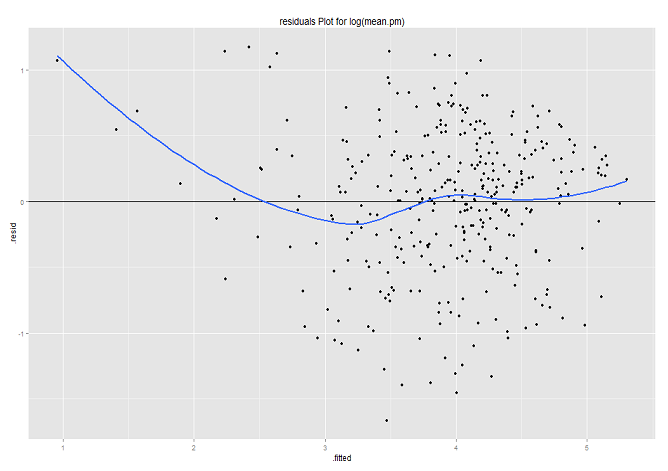
\includegraphics[width=0.6\textwidth]{Figure2-4}
      \caption{Residual plot of new fitted model after log transformation of daily average \(PM_{2.5}\). 18 outliers are still not included in the dataset.}
\end{figure}

\subsection{Exploring outliers with mean \(PM_{2.5} > 250\)}

 \begin{figure}[!ht]
  \centering
    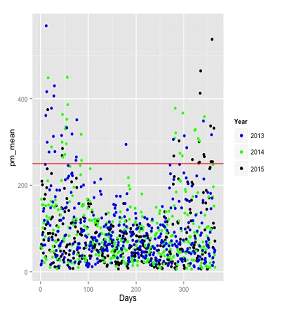
\includegraphics[width=0.6\textwidth]{Figure2-5}
      \caption{Daily averages for every day from 2013-2015--points from 2013 are displayed in blue, points from 2014 in green, and points from 2015 in black.}
\end{figure}

As can be seen in Figure 8 above, the outliers of 2015 were concentrated in January, Feburary, October, November, and December. These are the months when temperatures are relatively low within a year. Naturally, we want to see if this phenomenon holds across many years. So we looked at the three years of data from 2013 to 2015. Table 2 shows the results, which confirm the concentration of outliers in the October-February season.

\begin{table}[t]
\begin{tabular}{| ccc | ccc | ccc |}
\hline
\multicolumn{3}{|c|}{2013} & 
\multicolumn{3}{|c|}{2014} &
\multicolumn{3}{|c|}{2015} \\ \hline
Month & Day & Mean \(PM_{2.5}\) & 
Month & Day & Mean \(PM_{2.5}\) &
Month & Day & Mean \(PM_{2.5}\) \\ \hline
1 & 11 & 361.2 &1 & 16 & 448.4 &1 & 15 & 374.8 \\
1 & 12 & 568.6 &1 & 23 & 288.4 &2 & 14 & 268.5  \\
1 & 13 & 416.3 &2 & 14 & 299.7 &2 & 15 & 285  \\
1 & 14 & 299.5 &2 & 15 & 363.8 &10 & 6 & 267.7 \\
1 & 18 & 276.8 &2 & 16 & 264.8 &10 & 17 & 302.7  \\
1 & 23 & 378.1 &2 & 20 & 271 &11 & 14 & 259.3  \\
1 & 27 & 313 &2 & 21 & 330.4 &11 & 27 & 251.4  \\
1 & 28 & 406.4 &2 & 22 & 335.5 &11 & 28 & 300.5  \\
1 & 29 & 429.8 &2 & 23 & 296 &11 & 29 & 253.2 \\
1 & 30 & 277.9 &2 & 24 & 352.6 &11 & 30 & 412.8  \\ 
2 & 13 & 315 &2 & 25 & 449.8 &12 & 1 & 464.4  \\
2 & 24 & 332.9 &2 & 26 & 386.4 &12 & 8 & 270.9   \\
3 & 7 & 318.5&3 & 26 & 317.9 &12 & 9 & 266.2  \\
3 & 15 & 257.5 &3 & 27 & 257.4 &12 & 22 & 337   \\
3 & 16 & 265.2 &10 & 8 & 308.8&12 & 23 & 254.5  \\
3 & 17 & 351.3 &10  & 9 & 378 &12 & 25 & 537.2   \\
6 & 28 & 294.5 &10 & 10 & 321.1 &12 & 26 & 254.3  \\
10 & 5 & 306 &10  & 19 & 274 &12 & 29 & 331.9  \\
10  & 28 & 314.3 &10 & 25 & 267.8 &&& \\
11 & 2 & 286.8 &10  & 25 & 367 &&& \\
12 & 7 & 348.5  &11 & 19 & 327 &&& \\
12 & 24 & 316.8 &11 & 20 & 328.9 &&& \\
&&&11 & 26 & 308.9 &&& \\
&&&11 & 29 & 302.5 &&& \\
&&&12 & 9 & 358.6 &&& \\
\hline
\end{tabular}
\caption{Outliers with mean \(PM_{2.5} > 250\) in 2013-2015}
\end{table}

In the regression we performed above, there is a solid linear relationship between the \(PM_{2.5}\) values (excluding extreme values) and the meteorological variables. So we wanted to check if there's a linear relationship among the extreme values and the meteorological variables on those days. 
The fitted results are plotted in Figure 9 below.

 \begin{figure}[!ht]
  \centering
    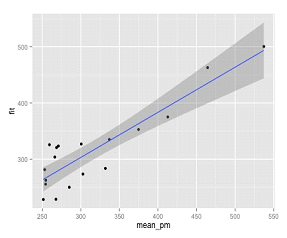
\includegraphics[width=0.6\textwidth]{Figure2-6}
       \caption{Fitted values of a linear regression for outliers in 2015.}
\end{figure}

Only one meteorological variable is significant, mean visibility (in miles). This variable imakes intuitive sense given the relation between air pollution and visibility. However, it's not really what we're interested in looking at. So I refitted the model without this variable. When the variable of mean visibility was removed, mean \emph{sea level pressure} became significant.

I could not find a good reason in my existing knowledge which would explain the relationship, but I was curious to see how strong this relationship was. So I decided to see if a similar relationship would hold throughout one particular day. 
So I took the 24 recorded \(PM_{2.5}\) values from January 15, 2015, which was an exceptionally bad day for emissions. On these 24 points I did a regression on the corresponding meteorological variables within the day. The regression result is shown in Figure 10. It turned out that again the sea level pressure was significant with a major adjusted R-square of 0.77.

 \begin{figure}[!ht]
  \centering
    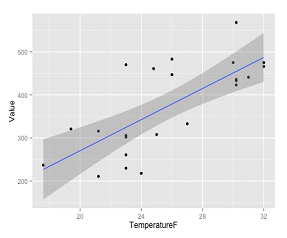
\includegraphics[width=0.6\textwidth]{Figure2-7}
      \caption{Fitted values of a linear regression for \(PM_{2.5}\) values on January 15, 2015.}
\end{figure}

\subsubsection{Some ideas about the relationship between \(PM_{2.5}\) and sea level pressure}

Why might this relationship hold? Based on what I was able to find, it seems that Beijing is affected by a meteorologiclal situation called an \textit{inversion}. An inversion is a phenomenon of wind that can prevent air pollutants from escaping. Beijing is surrounded by mountain ranges that lead to the inversion layer—cold air settles on top of a warmer air mass, trapping the pollutants inside \cite{Hawkins10}. In a normal situation, air temperature would decrease with altitude. Due to the fact that cold air is denser than warm air, the warmer air near the surface is forced upward and carries \(PM_{2.5}\) away. In contrast, Beijing’s near-surface air cools down much faster than the air high above at night, and this causes an inversion layer to form (shown in Figure 11 below). Colder air sticks to the surface and traps the \(PM_{2.5}\), which then accumulates in the city.


 \begin{figure}[!ht]
  \centering
    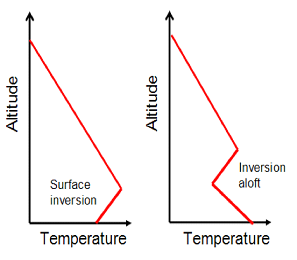
\includegraphics[width=0.6\textwidth]{Figure2-8}
      \caption{Relationship between Temperature and altitude\cite{Inversion}}
\end{figure}

According to the ideal gas law, we have \(PV=nRT\), and sea-level pressure is positively related to near-surface temperature.  
Near-surface temperature is minimal when the sea-level pressure is low and cold air would be trapped with \(PM_{2.5}\).
In conclusion, sea-level pressure should be negatively related to \(PM_{2.5}\) concentration.


\section{Conclusions and Future Work}

\subsection{General Comments}

Without an environmental expert to guide us through which research directions are more promising, 
it's difficult to do more than pattern-match. We can pattern-match and present the data well, but there's a major
limitation and inconvenience that comes from lacking expert domain knowledge.

From a technical perspective, 
it would be tremendously helpful to have someone who has expertise 
in hierarchical database management---in which hierarchical data is stored in a way 
that we can easily retrieve what we need and slice it up in more complicated ways.

Something else that might be worth effort by a research team or a company might be
to see which \(PM_{2.5}\) datasets are available for sites across the world.

Just as Beijing seemed to be a city with some
particular geographic features, are there other cities with similar accumulation footprints?

\subsection{Multi-Level Model}

One thing we saw as extremely promising along these lines was the massive climatological datasets that agencies like the NOAA collect.

In particular, the Reanalysis-2 dataset mentioned in the Data Sources section was incredibly rich--there were hundreds of readings
every month from dozens of locations. One of the things we wanted to build (but didn't have the time or background to do)
was a large multi-level, spatial model which would take data from all the sensors available to create a very precise idea
of the city's meteorological situation and could separate out city-specific, sensor-specific, time-specific contributions to variance
and determine what which the major local factors and patterns that could help us understand the sources and the sinks for
air pollution. 

The Reanalysis dataset likely would have been an undertaking of several months, if not years.
Much of the data was heavily nested and hard to access, much of it was missing, sensors seemed clustered around certain longitude lines,
many of the naming schemas were unclear, and overall, it would probably take a large amount of time and effort 
in conjunction with an expert to understand exactly how to use it.

On the other hand, for anyone who \emph{does} know how to use it, all relevant information is available.

\subsection{Meteorological Regression}

We haven't yet figured out the exact model for \(PM_{2.5}\) concentration on the meteorological factors, 
because we lack necessary prior knowledge and because we had trouble acquiring the data source. 
If we had more time on the project, we might find ways to deal with these problems and fit a much better model. 

So far, we have a sense that \(PM_{2.5}\) concentration does have relationship with meteorological data,
as the temperature, wind speed, and sea level pressure all seem to have negative impacts on the \(PM_{2.5}\) in Beijing, based on a daily average level of one year. 
However, we have no idea about other variables, such as precipitation and circulation. 

Thus, in the future, for the regression part, we want to find more explanatory predictors for the final model.
We would also like to explore the specific relationship between \(PM_{2.5}\) concentration and meteorological factors on an hourly level (if the right dataset is available). 

Moreover, we'd like to try to analyze the results using spatial data in order to compare the differences between regressions among cities.

\section{Data Sources}

As mentioned previously, the United States Department of State measures
air quality data at five locations---the U.S. Embassy in
Beijing, and the Consulates in Chengdu, Guangzhou,
Shanghai, and Shenyang. More detailed information about
the files and the data use statement can be found at www.stateair.net\cite{StateAirFS, StateAirDU}.

For the regression and outlier analyses, we obtained our meteorological data for Beijing (from the site "Weather Underground'' (at http://www.wunderground.com))
which contains temperature, dew-point, humidity, sea-level, pressure, visibility, and wind speed. This was used in our regression.

A dataset we weren't able to use---but is worth mentioning---
is the NCEP/DOE AMIP-II Reanalysis (Reanalysis-2) dataset 
from the National Oceanic and Atmospheric Administration
(NOAA)\cite{NOAA, NOAA2}, provided through 
the National Center for Atmospheric Research (NCAR). This was described in more detail in Part 3.

\subsection{Outliers:} 

For extreme air pollution events--besides sea level pressure, there must be other factors that will explain part of it, like coal usage during heating time if we can get the data. It’s a cumulative process that eventually result in an outlier. One idea is to find some relationship between one outlier and several days before it (as opposed to just the one-day lagged mean), and see if there is a trend or pattern for the outliers. 







\begin{thebibliography}{1}
\footnotesize

\bibitem{NOAA} National Centers for Environmental Prediction/National Weather Service/NOAA/U.S. Department of Commerce. 2000. NCEP/DOE Reanalysis 2 (R2). Research Data Archive at the National Center for Atmospheric Research, Computational and Information Systems Laboratory. http://rda.ucar.edu/datasets/ds091.0/. Accessed Feb. 24, 2015.

\bibitem{NOAA2} ``NCEP/DOE AMIP-II Reanalysis (Reanalysis-2)'' \textit{National Weather Service---Climate Prediction Center}. Accessed from web on Feb. 24, 2016.

\bibitem{StateAirFS} ``Fact Sheet,'' \textit{U.S.  Department of State}. Accessed from web on Feb. 24, 2016.
http://www.stateair.net/web/assets/USDOS\_AQDataFilesFactSheet.pdf

\bibitem{StateAirDU} ``Data Use Statement,'' \textit{U.S.  Department of State}. Accessed from web on Feb. 24, 2016.
http://www.stateair.net/web/assets/USDOS\_AQDataUseStatement.pdf

\bibitem{AQICN16} ``Revised PM2.5 AQI breakpoints,'' \textit{AQICN.org}. Accessed from web on Feb. 24, 2016.

\bibitem{Wiki16} 	``List of cities in China by population and built-up area,'' \textit{Wikipedia}. Accessed from web on Feb. 24, 2016.

\bibitem{Rohde15} Rohde, Robert A., and Richard A. Muller. "Air pollution in China: Mapping of concentrations and sources." \textit{PloS one}. 10.8 (2015): e0135749.

\bibitem{EPA16} ``Health | Particulate Matter | Air \& Radiation | US EPA,'' \textit{U.S. Environmental Protection Agency,''}. Accessed from web on Feb. 24, 2016.

\bibitem{WHO16} ``Metrics: Disability-Adjusted Life Year (DALY),'' \textit{World Health Organization}. Accessed from web on Feb. 24, 2016.

\bibitem{Yang10}
Yang, Gonghuan, et al. "Rapid health transition in China, 1990–2010: findings from the Global Burden of Disease Study 2010." \textit{The Lancet}. 381.9882 (2013): 1987-2015.

\bibitem{Stein14}
Stein, Rob. "China's Air Pollution Linked To Millions Of Early Deaths." \textit{NPR} 10 Feb. 2014. Accessed from web on Feb. 24, 2016.

\bibitem{Boren15}
Boren, Zachary D. "China Air Pollution: Beijing Records Its Cleanest Air Ever." \textit{Greenpeace}. 27 Aug. 2015. Accessed from web on Feb. 24, 2016.

\bibitem{Moore14}
Moore, Malcolm. "China's 'airpocalypse' Kills 350,000 to 500,000 Each Year." \textit{The Telegraph}. Telegraph Media Group, 07 Jan. 2014. Accessed from web on Feb. 24, 2016.

\bibitem{Chatani11}
Chatani, Satoru, Tazuko Morikawa, Seiji Nakatsuka, Sou Matsunaga, and Hiroaki Minoura. "Development of a framework for a high-resolution, three-dimensional regional air quality simulation and its application to predicting future air quality over Japan." \textit{Atmospheric Environment} 45, no. 7 (2011): 1383-1393.

\bibitem{Pohjola02}
Pohjola, M. A., A. Kousa, J. Kukkonen, J. Härkönen, A. Karppinen, P. Aarnio, and T. Koskentalo. "The spatial and temporal variation of measured urban PM10 and PM2. 5 in the Helsinki metropolitan area." \textit{Water, Air and Soil Pollution: Focus 2,} no. 5-6 (2002): 189-201.

\bibitem{Tai10}
Tai, Amos PK, Loretta J. Mickley, and Daniel J. Jacob. "Correlations between fine particulate matter (PM 2.5) and meteorological variables in the United States: Implications for the sensitivity of PM 2.5 to climate change." \textit{Atmospheric Environment} 44, no. 32 (2010): 3976-3984.

\bibitem{Inversion} Huber, Anna. ``Inversion Layers,'' \textit{csun.edu}. Aug. 26, 2004. Accessed from web on Feb. 24, 2016. 
Illustration sourced to [18]

\bibitem{Inversion2}
Turco, Richard P. Earth Under Siege: From Air Pollution to Global Change. New York: Oxford University Press, 2002. Print.

\bibitem{Hawkins10}
Hawkins, Timothy W., and Lisa A. Holland. "Synoptic and local weather conditions associated with PM2.5 concentration in Carlisle, Pennsylvania." \textit{Middle States Geographer} 43 (2010): 72-84.



\end{thebibliography}


\newpage



\textbf{Personal Statement}

\textit{Alex Dewey}

\paragraph{}Most of the groups I've ever been in tend to go in one of two general directions:

\begin{itemize}
\item One person takes control of the group, does by far the most work, and claims the most credit, or:
\item No one takes control of the group and the group doesn't find cohesion.
\end{itemize}

\paragraph{}From everyone I've ever spoken to, both experiences are pretty common. This group thankfully went much better than that. We genuinely approached problems as a group, we met to discuss specific roles, deadlines, and expectations, and while we all put effort into the group, no one tried to impose their specific vision.  We worked hard in this group, but we rarely overtaxed ourselves. We gave advice, but rarely gave commands. It was comfortable but not complacent. Cohesive but not stifling.

\paragraph{}We didn't really get a specific result from our project, and in terms of either the corporate or the academic world, that might be a problem in terms of funding or continuing a project. Indeed, we probably could have focused our efforts more on honing in on one specific question and answer, and how best to present our results in interesting ways , and that might have been helpful for getting something more at the end of the day. On the other hand, it strikes me that most meaningful progress on any non-trivial question of data science rarely takes just a few weeks, but is built on sustainable practices, realistic deadlines, good communication, and consistent progress over many months or even years. And that's something we did extremely well.

\paragraph{}There is a certain pressure to find a good-looking result in college and in business, which seems to be the major drive for ambitious people to take over groups. But those groups by their very nature are more prone to conflict than we were, learn less from one another than we did, and ultimately strike me as being much less satisfying and productive in the long term than we probably would be. Better the slow, inclusive search for a promising problem than the hasty, ambitious pursuit of the easy solution.

\paragraph{}One minor area we could have improved upon is to be a bit more forceful with pursuing our individual work and taken on a little more risk. We had three different promising threads for research, and we seemed hesitant to pursue any of them with too much vigor because none of us envisioned our individual projects as something we'd be able to present as a full project, and we wanted to be able to integrate our individual work with one another's, even though we never really developed a good plan for how we would integrate them. In the long term, that might have been a problem.

\paragraph{}Minor issues of coordination aside, the experience was extremely positive.
\end{document}


